\textbf{Remarks:}
\begin{align*}
    &
    \Phi^\intercal \vec{c} = \vec{y}
    \\&
    \Phi^\intercal \in \mathbb{R}^{(m+1) \times (n + 1)},\
    \vec{y} \in \mathbb{R}^{n+1},\
    \vec{c} \in \mathbb{R}^{m+1}
\end{align*}
is an overdetermined system (there are more equations than unknowns), if equations are independent.
Solution to least squares approximation provides the best approximate
solution to this system, with the error
\[
    \sum_{i=0}^n \Bigl(
        \sum_{j=0}^m c_j g_j(x_i) - y_i
    \Bigr)^2
\]

If we use a polynomial basis, we can ask, what is the best order of polynomial
for data that comes from a polynomial function (with observation error).
I.e. we have
\[ p_N(x) = \sum_{i=0}^N a_i x^i \]
without noise and $y = p_N(x) + \varepsilon$ as data with noise $\varepsilon$.

The variance of errors is from statistics:
\begin{align*}
    &
    \sigma_N^2 = \frac{1}{m - N} \sum_{i=0}^m \bigl(y_i - p_N(x_i)\bigr)^2
    \\&
    \sigma_0^2 > \sigma_1^2 > \dots > \sigma_N^2 = \sigma_{N+1}^2 = \dots = 
    \sigma_{m-1}^2
\end{align*}
We increase degree $N$ until $\sigma_N^2 \approx \sigma_{N+1}^2$.
This is polynomial regression.

\subsection{Differentiation and integration}
When analytical computations of derivatives are not possible, we resort to approximations.
\subsubsection{Difference quotients}
From calculus:
\[
    \lim_{h \to 0} \frac{f(x+h) - f(x)}{h} = f'(x)
\]
So, for $h$ small enough we may approximate
\[
    f'(x) \approx \frac{f(x+h) - f(x)}{h} \text{ --- \textbf{forward differencing}}
\]
How large is the error?
Taylor series expansion:
\begin{align*}
    &f(x+h) = f(x) + h \cdot f'(x) + \frac{h^2}{2} f''(\xi) \qquad \xi \in (x, x + h)
    \\&\iff
    f'(x) = \frac{f(x+h) - f(x)}{h} \textcolor{red}{- \frac{h}{2} f''(\xi)}
\end{align*}

Here $-\frac{h}{2} f''(\xi)$ is the exact error, asymptotically it's $\mathcal{O}(n)$.

What happens if we use
\[
    \lim_{h \to 0} \frac{f(x) - f(x-h)}{h} = f'(x) \text{ --- \textbf{backward differencing}}
\]
Error:
\begin{align*}
    &f(x - h) = f(x) - h f'(x) + \frac{h^2}{2} f''(\xi) \qquad \xi \in (x - h, x)
    \\&\iff
    f'(x) = \frac{f(x) - f(x - h)}{h} \textcolor{red}{+ \frac{h}{2} f''(\xi)}
    \\&
    \frac{h}{2} f''(\xi) = \mathcal{O}(h)
\end{align*}
\textit{Same} order as forward differencing.

Now take the two Taylor series expansions and subtract them:
\begin{align*}
    &
    f(x+h) = f(x) + hf'(x) + \frac{h^2}{2} f''(x) + \frac{h^3}{3!} f'''(\xi_1),\quad \xi_1 \in (x, x + h)
    \\&
    f(x-h) = f(x) - hf'(x) + \frac{h^2}{2} f''(x) - \frac{h^3}{3!} f'''(\xi_2),\quad \xi_2 \in (x, x + h)
    \\&
    f(x + h) - f(x - h) = 2h f'(x) + \frac{h^3}{3!} \bigl(f'''(\xi_1) + f'''(\xi_2)\bigr)
    \\&
    \iff f'(x) = \frac{f(x+h) - f(x-h)}{2h} \textcolor{red}{- \frac{h^2}{12} \bigl(f'''(\xi_1) + f'''(\xi_2)\bigr)}
    \\&
    f'(x) \approx \frac{f(x+h) - f(x-h)}{2h} \text{ --- \textbf{central differencing}}
    \\&
    \frac{h^2}{12} \bigl(f'''(\xi_1) + f'''(\xi_2)\bigr) = \mathcal{O}(h^2) \text{ --- error}
\end{align*}

\begin{figure*}[h]
    \centering
    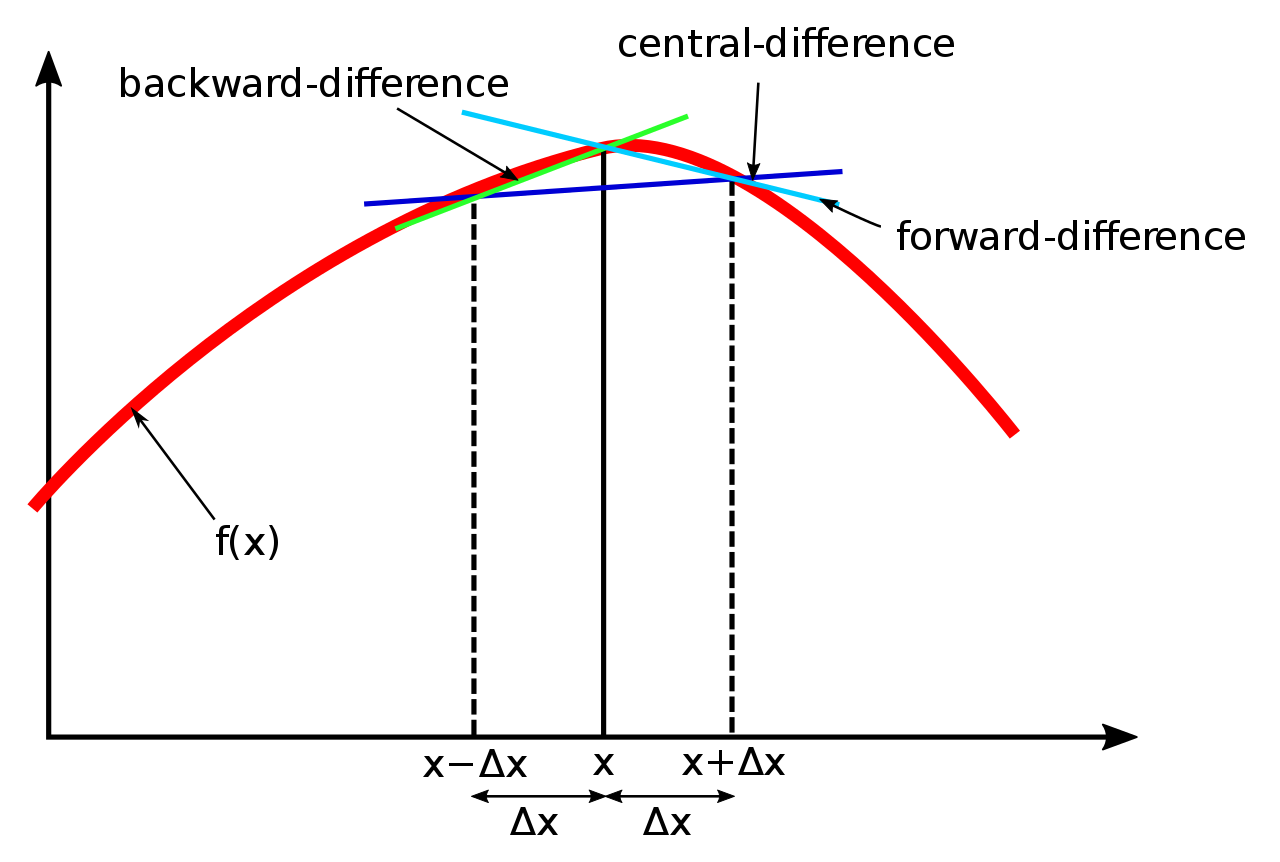
\includegraphics[width=0.7\textwidth]{differences}
\end{figure*}

\subsubsection{Richardson extrapolation}
Approach for producing higher order approximations from lower order approximations.

Suppose we have a low order approximation $\varphi(h)$ of a derivative, e.g.
\[
    f'(x) = \varphi(h) + a_1 h + a_2 h^2 + a_3 h^3 + \dots
\]
$\varphi(h)$ may be equal to the first order forward differencing:
\[
    \varphi(h) = \frac{f(x+h) - f(x)}{h}
\]
Alternatively, for central differencing we have:
\[
    \varphi(h) = \frac{f(x+h) - f(x-h)}{2h}
\]

\begin{example}
    For central differencing:
    \[ f'(x) = \varphi(h) + a_2 h^2 + a_4 h^4 + a_6 h^6 + \ldots = \text{(1)} \]
    \textit{Trick:} evaluate for $h = \frac{h}{2}$
    \begin{align*}
        f'(x) &= \varphi\Bigl(\frac{h}{2}\Bigr) + a_2 \Bigl(\frac{h}{2}\Bigr)^2 + 
        a_4 \Bigl(\frac{h}{2}\Bigr)^4 + a_6 \Bigl(\frac{h}{2}\Bigr)^6 + \dots
        \\&
        = \varphi\Bigl(\frac{h}{2}\Bigr) + \frac{a_2}{4} h^2 + \frac{a_4}{16} h^4 + \frac{a_6}{64} h^6 + \ldots
        = \text{(2)}
    \end{align*}
    The idea is to combine (1) and (2) so that the low order terms cancel out.
    \begin{align*}
        &\text{(1)} - 4 \cdot \text{(2)} =
        \varphi(h) - 4 \varphi\Bigl(\frac{h}{2}\Bigr) + a_4\Bigl(1 - \frac{4}{16}\Bigr) h^4 + 
        a_6 \Bigl(1 - \frac{4}{16}\Bigr) h^6 + \dots
        \\&\iff
        -3f'(x) = \varphi(h) - 4 \varphi\Bigl(\frac{h}{2}\Bigr) + a_4 \frac{3}{4} h^4 + a_6 \frac{15}{16} h^6 + \dots
        \\&\iff
        f'(x) = \frac{4 \varphi\bigl(\frac{h}{2}\bigr) - \varphi(h)}{3} \textcolor{red}{- \frac{a_4}{4} h^4 - 
        a_6 \frac{5}{16} h^6 - \dots}
    \end{align*}
    The \textcolor{red}{error} is asymptotically $\mathcal{O}(h^4)$.

    So, the new approximation is
    \[ f'(x) =  \frac{4 \varphi\bigl(\frac{h}{2}\bigr) - \varphi(h)}{3} \]
    In particular, if we substitute $\varphi$ with the
    central differencing, we get
    \[
         f'(x) \approx \frac{f(x-h) - 8f\bigl(x - \frac{h}{2}\bigr) + 
         8f\bigl(x + \frac{h}{2}\bigr) - f(x+h)}{6h}
    \]
\end{example}

The process of halving the step size and cancelling out terms of the error
can be repeated!
We got better approximation at the price of more lower order terms in 
the approximation formula.

For polynomials, the right order Richardson extrapolation will be exact,
as higher order derivatives are zero.

\subsubsection{Higher order derivatives}
Again, we use Taylor series:
\begin{align*}
    &
    f(x+h) = f(x) + hf'(x) + \frac{h^2}{2} f''(x) + \frac{h^3}{3!} f'''(x) 
    + \frac{h^4}{4!} f''''(\xi_1) \quad \xi_1 \in (x, x + h)
    \\&
    f(x - h) = f(x) - hf'(x) + \frac{h^2}{2} f''(x) - \frac{h^3}{3!} f'''(x) 
    + \frac{h^4}{4!} f''''(\xi_2) \quad \xi_2 \in (x - h, x)
\end{align*}
We want to cancel $f'(x)$. For that we can simply add the two series:
\begin{align*}
    &f(x + h) + f(x - h) = 2f(x) + h^2 f''(x) + \frac{1}{4!} h^4 \bigl(
        f''''(\xi_1) + f''''(\xi_2)
    \bigr)
    \\&\iff
    f''(x) = \frac{f(x+h) - 2f(x) + f(x-h)}{h^2}
    \textcolor{red}{- \frac{1}{4!} h^2 \bigl(f''(\xi_1) + f''(\xi_2)\bigr) }
\end{align*}
Here we are using the 3 point stencil (i.e. we need three neighboring points:
$x - h$, $x$, $x+h$), and the weights are $[1, -2, 1]$.
The \textcolor{red}{error} is of order $\mathcal{O}(h^2)$.

Again, Richardson extrapolation can be used to get a better approximation.

\pagebreak
\subsubsection*{Summary of numerical derivatives:}
\begin{itemize}
    \item {
        Backward difference quotient, $\mathcal{O}(h)$.
    }
    \item {
        Forward difference quotient, $\mathcal{O}(h)$.
    }
    \item {
        Central difference quotient, $\mathcal{O}(h^2)$.
    }
\end{itemize}
Taylor series expansion is used for error analysus.

Richardson extrapolation: use approximation $\varphi$ for $h$ and $\frac{h}{2}$.
Combine $\varphi(h)$ and $\varphi\bigl(\frac{h}{2}\bigr)$ such that
the low order error terms cancel out, e.g. for central differencing.
\[
    \frac{4 \varphi\bigl(\frac{h}{2}\bigr) - \varphi(h)}{3}
    \text{ is } \mathcal{O}(h^4)
\]

\subsection{Integration/Quadrature rules}
We need numerical integration when anti-derivatives cannot be found easily.

From calculus: assume $f \ge 0$ integrable, $f : [a, b] \to \mathbb{R}$.
\subsubsection{Riemann sums}
\begin{enumerate}
    \item {
        Partition $P$ of $[a, b]$. Introduce nodes
        $a = x_0 < x_1 < \dots < x_n = b$ (discretize continuous interval)
        and sub-intervals $[x_i, x_{i+1}]$, for $i = 0, \dots, n - 1$.
        \begin{center}   
            \begin{tikzpicture}
                \begin{axis}[
                    axis x line=left,
                    axis y line=none,
                    axis line style={-{Stealth[scale=1.5]}},
                    xtick={0, 1, 2, 3, 4, 5, 6},
                    xticklabels={$a$, $ $, $ $, $ $, $ $, $ $, $b$},
                    ytick=\empty,
                    xmin=-0.5, xmax=6.5, ymin=0, ymax=1
                ]\end{axis}
            \end{tikzpicture}
        \end{center}
        \begin{figure*}[h]
            \centering
            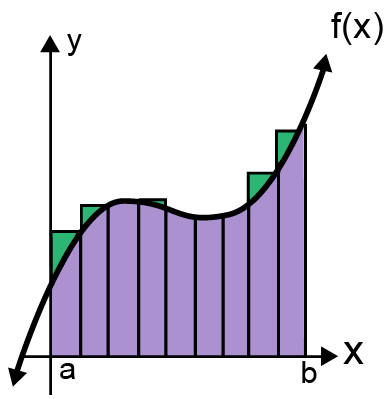
\includegraphics[width=0.25\textwidth]{riemann}
        \end{figure*}
    }
    \item {
        Approximate area under curve by summing up areas of rectangles. \textbf{Riemann sum:}
        \[
            \sum_{i=0}^{n-1} (x_{i+1} - x_i) f(x_i^*) \quad x_i^* \in [x_i, x_{i+1}]
        \]
        Here $x_{i+1} - x_i$ is the width, and $f(x_i^*)$ is the height.
    }   
    \item {
        If $f$ is continuous, then $x_i^*$ may be chosen arbitrarily in $[x_i, x_{i+1}]$.
        Two choices are interesting:
        \begin{enumerate}
            \item {
                $x_i^*$ such that $f(x_i^*) = \min\{ f(x) \mid x_i \le x \le x_{i+1} \} =: m_i$
            }
            \item {
                $x_i^*$ such that $f(x_i^*) = \max\{ f(x) \mid x_i \le x \le x_{i+1} \} =: M_i$
            }
        \end{enumerate}
    }
    \item {
        Then, 
        \begin{align*}
            &
            L(f; P) = \sum_{i=0}^{n-1} (x_{i+1} - x_i) \cdot m_i \text{ --- \textbf{lower sum}}
            \\&
            U(f; P) = \sum_{i=0}^{n-1} (x_{i+1} - x_i) \cdot M_i \text{ --- \textbf{upper sum}}
            \\\implies
            &L(f; P) \le \int_a^b f(x) \,dx \le U(f; P)
        \end{align*}
    }
\end{enumerate}

Some integrations are straight-forward, e.g.:
\[
    f(x) = x^2 \quad \int_a^b f(x)\,dx = \frac{b^3}{3} - \frac{a^3}{3}
\]
But we need numerical methods to find
\[ \int_a^b e^{x^2} \,dx \]
We cannot find an analytical solution consisting of elementary functions. That does not mean
that the function is not integrable!
